\documentclass[12pt]{article}

%
%Margin - 1 inch on all sides
%
\usepackage[letterpaper]{geometry}
\geometry{top=1.0in, bottom=1.0in, left=1.0in, right=1.0in}

%
%Doublespacing
%
\usepackage{setspace}
\doublespacing

% 
%Babel package for multiple language typesetting
%
%\usepackage[english,spanish]{babel}
%\usepackage[T1]{fontenc}
%\usepackage[latin1]{inputenc}

%
%Setting the font
%G
\usepackage{times}
\usepackage{graphicx}

\renewcommand{\thesection}{\arabic{section}.}

%
%Works cited environment
%(to start, use \begin{workscited...}, each entry preceded by \bibent)
% - from Ryan Alcock's MLA style file
%
\newcommand{\bibent}{\noindent \hangindent 40pt}
\newenvironment{workscited}{\newpage \begin{center} Works Cited \end{center}}{\newpage }

\newcommand{\mc}{M\'airt\'in}
\newcommand{\mcs}{M\'airt\'in }

%
%Begin document
%
\begin{document}
\begin{flushleft}

%%%%First page name, class, etc
Michael Gilliland \\
Dr. Linda Szabo \\
Humanities 203 \\
\today \\
Words: 1395 \\

%%%%Title
\begin{center}
{\large The Propitious Drones from Nevada}
\end{center}

%%%%Changes paragraph indentation to 0.5in
\setlength{\parindent}{0.5in} 

%START%

\section{Description of Characters and Obstacles}

\indent Although it is only briefly mentioned in \emph{The Odyssey} by Menelaus, the story of
the Trojan Horse, a technological marvel in which Odysseus and other Grecians hid to defeat the Trojans,
is a legend of Greek heritage that I have marveled at since I was a child (Fagles 133).
Technology has captivated me my entire life, and because of this, technology (specifically regarding the question of
whether it is a benefactor or opponent of society) is the primary theme of my epic entitled \emph{The Propitious
Drones from Nevada}. My plot's hero has an interest
in technology, but questioningly so. This hero's name is \mcs Ashley.

\mc, a 25 year-old, modernist architect living in Henderson, Nevada, possesses a lifelong urge
to make the world a better place and -- through doing so -- better himself. Physically, \mcs is somewhat common. 
He is slim, and slightly petite with a dark complexion and long, brown hair. He is an extremely curious individual
who will always seek out his own answers and, by his efforts, has gained a magnitude of endurance that withstands
the adversity of "luck," interaction and situation. \mc's greatest quality, the primary instance of which is yet to be 
revealed, is sacrifice. Looking at the world around him, \mcs sees pain and toil; his qualities are in direct revolt to these
problems. They are his intentional attempt to solve them. \mcs will soon find that the world's problems
are much greater than he ever could have ever expected.

There are two main obstacles that \mcs will face in his journey. The first, as will be further described in the plot summary,
occurs by accident. \mcs must endure the desert, hiking thirstily while weary, bloody and bruised; without the satisfaction
of nourishment. Secondly, \mcs will have to face two drones (evil robots) each led by its synthetic, emulated
will. Another drone, called Gamma serves as a companion to \mc, as well as an antithesis to the depraved drones.
Gamma possesses the will of the scientist who was the fountainhead of the technology by which the drones were
engendered.

\section{Ten Opening Lines}

Alas, the soulless night-owls perch atop the globe; the very images of patriotic affluence, of beloved charity.
They need not take power, for to them we have freely given all authority, to these devils we have exchanged our very
souls for naught but the dirt which we will one day call \emph{home}.
Their clanking bones collide beneath synthetic skin, never-breaking, indifferent to the strains of time.
The spoked axle that is their heart, rotates perpetually, powered by the invisible desire of sub-microscopic slaves,
indebted to an unattainable hope. Who will make the world anew? Who possesses the ability to raze the dormant principality whose
power resides in its patience, whose war is waged in peace and whose visible love encapsulates a masked hatred.
In the world there is peace -- the night sleeps -- they do not. Their effort is dedicated to gaining prominence,
to secretly colonizing in the dark. In this epoch of emulated prosperity, who can make the world anew?

\section{Plot Summary}

As the plot opens, \mcs Ashley is driving his Oldsmobile from his home at Henderson
to Vegas. Some weekends, he drives to Vegas to practice his draftsmanship by sketching some of
the architectural wonders thereabout. As he enters the city, he sees a curious sight out his car window: 
a woman being dragged out of a casino by men wearing dark suits. He indulges 
his curiosity for a moment when, \emph{WHAM!} He crashes into a limousine in front of him.
A few men with dark suits rush out of the posteriorly mangled limo.

Realizing that these individuals do not appear to have his best interest in mind and that a
dark smoke is beginning to emit from his car's hood, \mcs promptly departs his vehicle.
Abruptly he is stopped, seeing nothing but a red and
black striped tie as his face is forcefully planted upon the upper chest of a flanking pursuer. 
\mcs backs away. He looks
around, noticing about a half-dozen suit wearing mobster type figures. One of the mobsters shouts an insult
at him.
\mcs tries to curb them with words
implying passive reaction. He finds no success. Unable to defend himself from the aggressors,
they beat him down, lacking mercy or any inclination of humane remorse.

\mcs awakes to the sound of a low rumbling, in the trunk of a car.
Over the sound of the engine, he makes out words from a deep voice -- the 
aggressor who had shouted earlier. "The boss said that...," \mcs hears. Then, a few moments later, "...near
the border of Arizona and Nevada...." \mcs lays back, drifting 
into sleep. He experiences an eccentric sense of comfort or (perhaps) just delusion. 

The unpleasant amalgamation of a creaking noise and a bright light awakening him this time, \mcs sees
the shouter who then pulls him out of the trunk, throws him on the ground, gives him a kick in the
side and informs \mcs in pure sarcasm, "We gotta special treat for you today. For screwin'
up the boss' favorite limo, you get to be buzzard food." \mcs stares silently. An act which disturbes the heart of
the mobster who had never felt such a calm as \mcs illuminated. "Well, if you got nothin' to say," said the mobster 
shakingly, "So long."

\mcs stood as the mobster drove off. He saw no rodes, his cell phone was taken, but,
since it was not yet night -- he would walk West. He endured the desert for a long time, stopping
occasionally to eat safe plants he found and to rest. As he is walking near a mountain, the ground starts
shifting below him, he stumbles and falls down a trap hatch hidden in the desert.

Cushioned by the sand that falls with him, \mcs looks around at his new surroundings \mcs sees
a dark laboratory. The first thing that catches his eye is a flickering computer screen with a window open (Revelation 1). Next,
he sees a palm-sized circuit board. The strange board is labeled "RVC No. 3" (Revelation 2). The third
thing he finds is a robot, with glowing eyes and an empty port on the side of its head, into which he inserts the RVC
(Revelation 3).
The robot comes to life and begins to tell a story of a scientist and a politician.

About a decade ago, the great scientist, under the sponsorship of Benjamin Spade (the politician) had created a machine
that could import the will of any living organism into a circuit card known as the \emph{Replicated Volition Chip}.
\mcs had heard of Spade, in fact, there was hardly day when he could go without hearing about the increasingly
prominent politician. The robot proceeds to tell \mcs that the chips could be implanted into drones that would then act out
the will within the RVC. It then explains that the first RVC contained a mixture of the wills of many animals and the will of 
a criminal. The second contained Spade's
will.

Continuing, almost sorrowfully the drone tells \mcs that the scientist saw an unnatural evil in the wills of Spade and the
animals and that, in desperation, he secretly uploaded his own will into the third RVC, along with the account that
is currently being relaying. The remorseful drone then went on to say that the great scientist had given the drones the ability
to mask themselves (to the human eye) as the original bearer of their possessed will, and that they had been programmed in such a way that they
were unable to download different or new wills. With almost human sadness in his voice, the drone
finished his account, saying that the animal drone and Spade's drone turned on them, killing Spade and the great scientist.
"They will not stop," the drone concluded, "Until they have acclimated themselves into society with such prominence that
they can destroy it. Then they will deconstruct this world."

After the sobering account, the drone brings \mcs some canned food that had been left in the lab and it introduces itself
as \emph{Model Gamma}, saying, "Nowhere in the account did the scientist provide his name." \mcs and
Gamma (now masked as the great scientist) make their way, through an underground tunnel system revealed by Gamma, to
a small town in Eastern Nevada from which they take a bus back to \mc's home. At \mc's house, they research Spade to
learn the location of the imposter (in truth a masked drone,)
discovering that he will be speaking in Vegas later that week. That is when they decide to strike.

Later, at the drone's speech, as soon as it begins speaking, Gamma points out the animal-willed drone, now acting
as one of Spade's numerous bodyguards. Then, they sprint out from the crowd,
Gamma at Spade and \mcs at the animal-willed. As \mcs begins beating the drone with the baseball bat he brought along for the
occasion, he sees metal and sparks shooting from Gamma and Spade as they clash. Bullets fly through Gamma from every side
but Gamma keeps fighting on until he alone arises victorious, standing convoluted over his defeated opponent. \mc, has an advantage over
the animal-conglomerate-being, because he struck in surprise. He also destroys his enemy, taking his final blow at
the criminal-animal drone's RVC. The surge of victory he feels is only matched by
a surge of pain. Looking down he sees blood smeared over his chest, the effect of bullets from nearby bodyguards. He falls to the
floor and his new found friend, Gamma the drone, picks him up and flees the scene bearing the body of he who sacrificed
so much for the people of this world.

%END%

\section{The Hero's Revelations}

\noindent  
\includegraphics[scale=0.5]{RVCWindow.png} \\
\noindent  {\bf Revelation 1: RVC Window}
\newline

\noindent  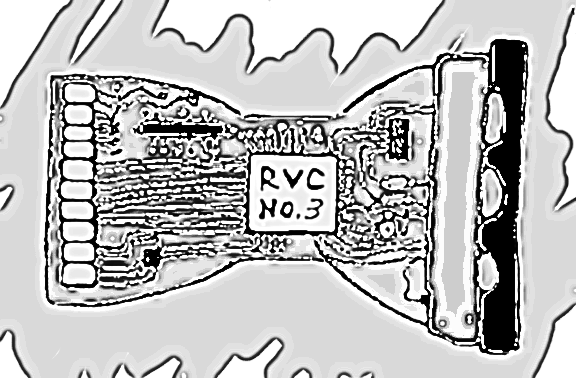
\includegraphics[scale=0.75]{RVC_BAW.png} \\
\noindent  {\bf Revelation 2: The Third Replicated Volition Chip}
\newline

\noindent  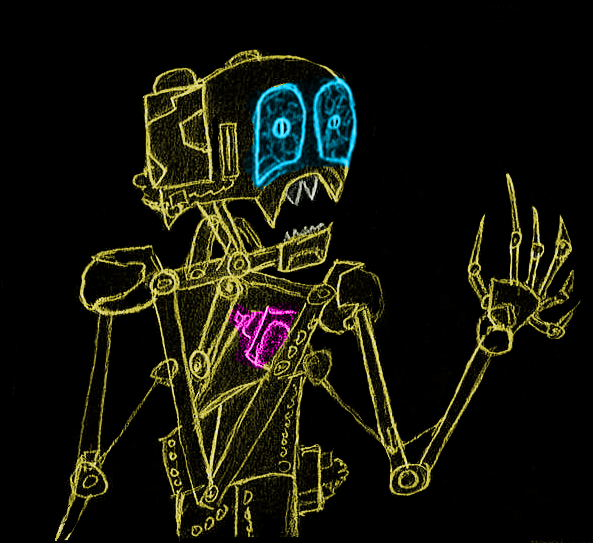
\includegraphics[scale=0.75]{Drone_InDark.png} \\
\noindent  {\bf Revelation 3: Gamma in the Dark}


%%%%Works cited
\begin{workscited}

\bibent
Homer, and Robert Fagles. \textit{The Odyssey}. New York: Penguin, 1997. Print.

\bibent
Gilliland, Michael. "RVC Window in PyGTK". 2013. PNG file.

\bibent
Gilliland, Michael. "The Third RVC". 2013. PNG file.

\bibent
Gilliland, Michael. "Model Gamma in the Dark". 2013. PNG file.

\end{workscited}

\end{flushleft}
\end{document}
\}

